\documentclass{article}

\usepackage[preprint]{neurips_2026}

\usepackage[utf8]{inputenc}
\usepackage[T1]{fontenc}
\usepackage{hyperref}
\usepackage{url}
\usepackage{booktabs}
\usepackage{amsfonts}
\usepackage{nicefrac}
\usepackage{microtype}
\usepackage{xcolor}
\usepackage{graphicx}
\usepackage{enumitem}
\usepackage{amsmath}

\title{Benchmarking and Adapting Open-Source Vision-Language Models for TextVQA: A Funnel Evaluation and LoRA Fine-Tuning Study}

\author{%
  Chenxi Ge \And Harry Hu \\
  Harvard University, School of Engineering and Applied Sciences \\
  \texttt{steven\_ge@fas.harvard.edu, harryhu@fas.harvard.edu}
}

\begin{document}

\maketitle

\begin{abstract}
TextVQA requires a model to read scene text, ground it in visual context, and answer natural-language questions with high exact-match precision. Although open-source vision-language models (VLMs) have improved rapidly, rigorous TextVQA studies still face a practical tension between benchmark breadth, adaptation depth, and limited compute. We address this problem with a staged empirical protocol that combines broad zero-shot screening, disciplined finalist reruns, and winner-conditioned LoRA fine-tuning within a single reproducible pipeline. The study benchmarks four open-source VLM families and an OCR lexical baseline, uses a stratified internal development split to preserve the official validation set for serious comparisons, and separates training-stage family selection from post-training accuracy-based model promotion. The resulting design is deliberately structured to produce interpretable model comparisons, defensible adaptation decisions, and reproducible evidence under a realistic compute budget while retaining enough experimental breadth to support a substantive analysis of OCR usage, prompt sensitivity, and parameter-efficient adaptation.
\end{abstract}

\section{Introduction}

Reading text in natural images remains a central failure mode for otherwise capable vision-language systems. The TextVQA benchmark was introduced precisely to stress this gap: a successful model must not only parse scene text, but also integrate it with visual context and question semantics to produce a short, exact answer \citep{singh2019textvqa}. In practice, this setting is harder than generic image question answering \citep{antol2015vqa} because many correct responses depend on OCR fidelity, prompt format, answer normalization, and the model's ability to reason over text that is sparse, noisy, or visually embedded in cluttered scenes.

At the same time, the open-source VLM ecosystem has matured enough that a serious empirical study is now feasible without closed commercial models. Architectures such as BLIP-2 \citep{li2023blip2}, LLaVA \citep{liu2023visual}, InternVL2.5 \citep{chen2024internvl25}, and Qwen2.5-VL \citep{qwen2025qwen25vl} offer strong multimodal priors at parameter scales that can still be evaluated and adapted in an academic setting. Yet the existence of capable models does not, by itself, solve the experimental-design problem. A naïve study can easily become either too shallow, by comparing only a small number of zero-shot settings, or too diffuse, by mixing screening, validation, prompt exploration, and fine-tuning without a clear promotion policy. In TextVQA, where OCR choices matter almost as much as backbone choice, such looseness makes the final conclusions difficult to defend.

This paper therefore adopts a deliberately staged protocol rather than a flat benchmark. We first run broad zero-shot screening on a stratified internal development split, then reserve the official validation set for a narrower set of finalists, and finally conduct a winner-conditioned LoRA study on the selected backbone. The key principle is that each stage should answer a different scientific question: screening compares backbones and OCR-sensitive prompting cheaply, finalist reruns verify which combinations are still competitive on the official split, and the training stage isolates the effect of parameter-efficient adaptation while keeping follow-up ablations attached to a selected LoRA family rather than to an arbitrary default. The final claims are made on official validation evidence, while internal-dev results are used for screening, diagnostics, and budget allocation. The result is an experiment that is broader than a single-tuned-model class project, but still structured enough to remain methodologically coherent.

Our study is also designed around realistic compute constraints rather than idealized cluster access. All canonical evaluation runs are executed locally in a resumable queue on a single Apple-Silicon workstation, while only the final LoRA matrix is moved to rented remote GPUs under a separate run namespace. This separation is not merely operational. It preserves a clean experimental boundary between the local zero-shot/finalist evidence and the remote training evidence, reducing the risk that nominally identical runs mix hardware regimes, caches, or checkpoints in ways that complicate interpretation.

The paper makes the following contributions. First, it introduces a reproducible funnel protocol for benchmarking open-source VLMs on TextVQA while preserving the official validation split for finalist and final tuned-model evidence. Second, it treats OCR as a first-class experimental variable across zero-shot prompting, training-time ablation, and post-hoc robustness analysis. Third, it develops a winner-conditioned LoRA study in which training-stage follow-up allocation, internal-dev adapter promotion, and official-validation claims are explicitly separated. This separation keeps a local diagnostic objective distinct from the final paper-facing evaluation objective. Finally, the project delivers a complete implementation pipeline that couples layered configuration, resumable execution, remote multi-GPU orchestration, progress reporting, and generated audit artifacts, making the empirical claims auditable rather than anecdotal.

Section~\ref{sec:related} situates the study with respect to TextVQA, open-source VLMs, and parameter-efficient adaptation. Section~\ref{sec:design} then formalizes the staged experimental protocol and systems boundary that govern the full study.

\section{Related Work}
\label{sec:related}

\subsection{TextVQA and text-grounded visual question answering}

TextVQA was introduced to measure a model's ability to answer questions whose solution depends on reading text embedded in real-world images \citep{singh2019textvqa}. Unlike generic VQA, the benchmark frequently requires exact recognition of sparse text, reasoning over OCR tokens, and answer generation under strict string-matching evaluation. This makes the problem particularly sensitive to small prompt decisions, OCR formatting, and answer normalization. For an empirical paper, the implication is straightforward: a convincing TextVQA study must treat text handling as part of the research question rather than as an implementation footnote.

That requirement shapes the present study in two ways. First, OCR-aware prompting is treated as a structured experimental variable throughout zero-shot evaluation rather than as a single fixed preprocessing choice. Second, OCR remains part of the fine-tuning analysis through explicit on/off follow-up runs. This design choice is motivated by the benchmark itself: if scene text is central to the task, then conclusions about backbone quality or adaptation quality are incomplete unless OCR usage is interrogated directly.

\subsection{Open-source vision-language models}

Open-source VLMs have advanced rapidly through increasingly effective combinations of pretrained vision encoders, pretrained language models, and instruction-tuning pipelines. BLIP-2 demonstrated that strong multimodal transfer can be achieved by bootstrapping from frozen unimodal components rather than retraining the full stack from scratch \citep{li2023blip2}. LLaVA showed that visual instruction tuning can substantially improve general-purpose multimodal behavior with a comparatively lightweight alignment stage \citep{liu2023visual}. More recent model families, including Qwen2.5-VL \citep{qwen2025qwen25vl} and InternVL-style systems, have pushed open-source multimodal performance far beyond early proof-of-concept systems, making it realistic to benchmark several families within one study.

However, strong checkpoints alone do not guarantee a rigorous comparison. Public model reports typically emphasize aggregate benchmark leaderboards, while a project like ours must instead decide how to compare models under a fixed, transparent protocol. In particular, an academic benchmark on TextVQA must choose how much prompt breadth to allow, which split should be used for screening, and when it is appropriate to spend the official validation budget. Our funnel design can be understood as a methodological answer to that problem: broad internal-development screening is used to expose prompt and backbone sensitivity, while the official validation split is deliberately held back for a much smaller set of finalists and final tuned-model checks.

\subsection{Parameter-efficient adaptation}

The fine-tuning stage in this project is built around Low-Rank Adaptation (LoRA) \citep{hu2022lora}, which remains the most practical parameter-efficient adaptation method for a study that aims to compare several adaptation settings rather than optimize a single maximal model. LoRA is especially appropriate here for three reasons. First, it makes a multi-run ablation feasible within a limited compute budget. Second, it allows adaptation choices such as target-module strategy and rank to be varied systematically. Third, it keeps the training question close to the paper's actual scope: we are not trying to establish a new state of the art on TextVQA, but rather to understand how far a strong open-source backbone can be pushed under a controlled and reproducible adaptation budget.

Most importantly, we treat LoRA not as a one-off fine-tuning step but as a structured study. The core matrix compares attention-only and all-linear target strategies, rank $16$ versus $32$, and seed stability. The follow-up runs then ask higher-level questions that the core matrix alone cannot answer: whether OCR conditioning materially changes adapted performance, and whether additional data continues to improve the selected family. This winner-conditioned design is more informative than a single tuned checkpoint and more defensible than ablations attached to a family that never actually won the initial training comparison.

\section{Study Design and Experimental Protocol}
\label{sec:design}

\begin{figure*}[t]
    \centering
    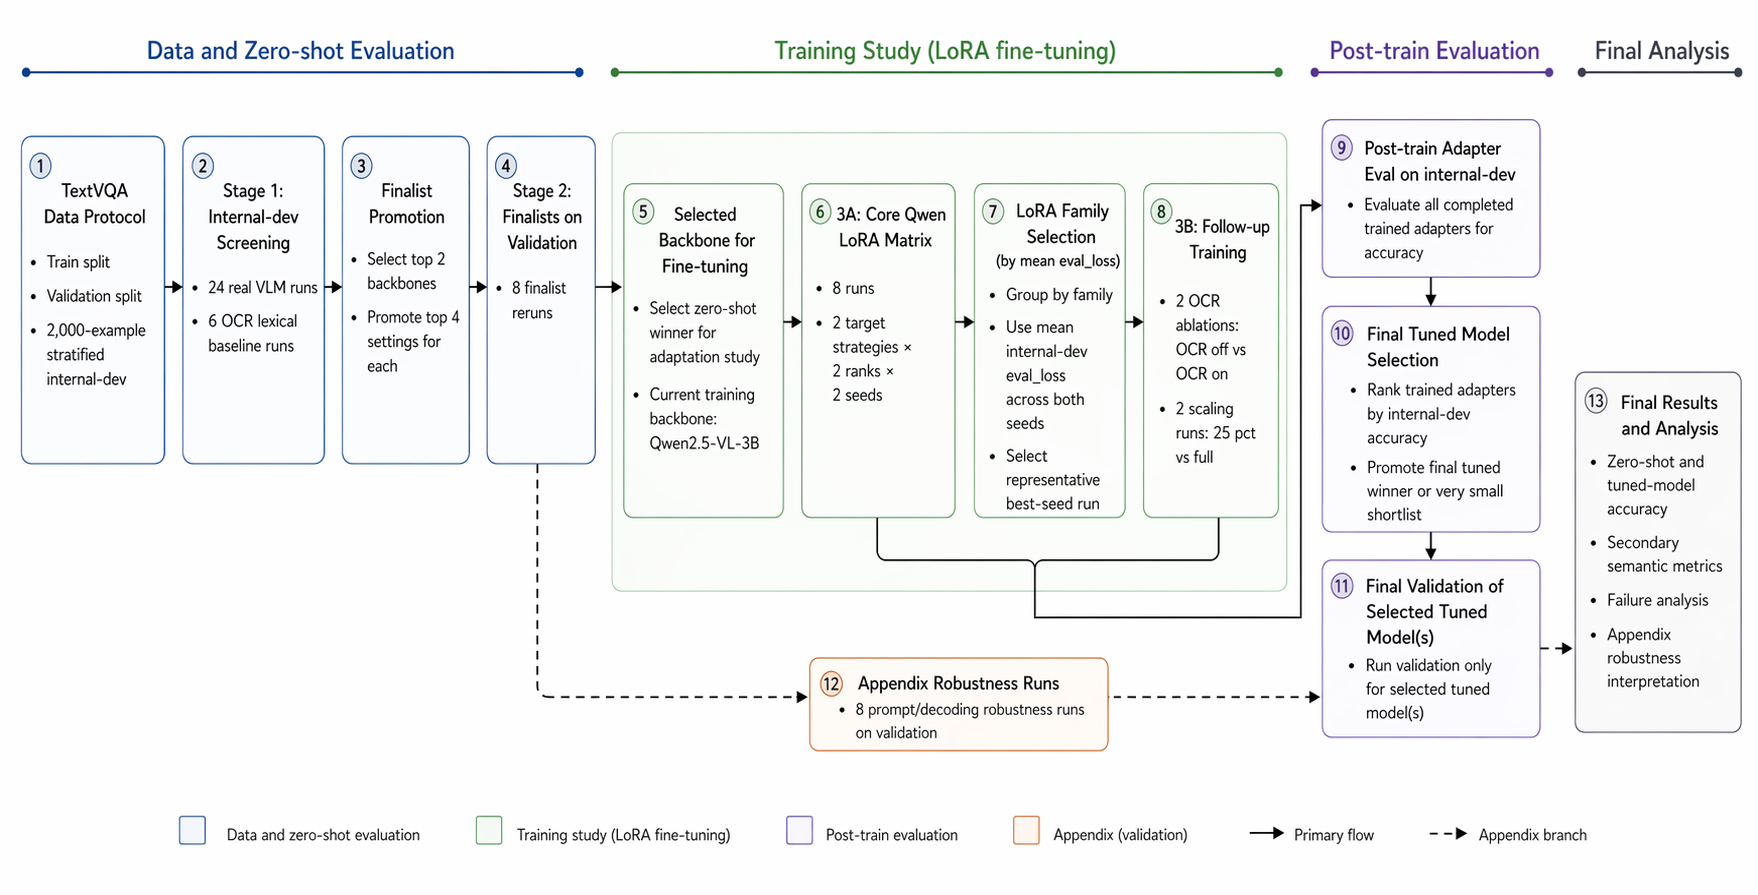
\includegraphics[width=\textwidth]{figures/textvqa_experiment_pipeline.png}
    \caption{End-to-end experiment pipeline for the current TextVQA study. The protocol follows a staged funnel: stratified internal-dev screening, finalist reruns on the official validation split, backbone selection for LoRA fine-tuning, an $8$-run core Qwen LoRA matrix, and $4$ winner-conditioned follow-up training runs. Training follow-ups are chosen by mean internal-dev \texttt{eval\_loss} across core seeds, whereas completed trained adapters are later ranked by internal-dev accuracy before promoting only the final tuned model, or a very small shortlist, to validation. Appendix robustness runs remain a secondary validation branch that supports the final analysis without altering the main winner-selection funnel.}
    \label{fig:pipeline}
\end{figure*}

\subsection{Task and data protocol}

The study follows the official TextVQA split structure of approximately $34.6$k training examples, $5$k validation examples, and $5.73$k test examples \citep{singh2019textvqa}. We reserve the official validation split for finalist reruns, appendix experiments, and final tuned-model checks. The test split is present in the local Hugging Face cache, but its answer fields are blank in this public release, so local test accuracy cannot be computed without submitting predictions to an external evaluation server. All paper-facing accuracy claims are therefore made on the official validation split, which is the highest-labeled held-out split available inside the reproducible artifact. To avoid using that validation split for broad exploratory screening, we materialize a separate $2{,}000$-question internal development set from the training split. This internal-dev set is stratified rather than sampled naively, with explicit control over question prefix, answer-length bucket, and OCR-token-count bucket. The remaining training questions form the training pool for the LoRA study.

The internal-dev split is question-disjoint from the LoRA training pool, but it is not fully image-disjoint: TextVQA contains multiple questions for some images, and the current split removes selected questions rather than every question attached to the same image. Table~\ref{tab:split-audit} makes this boundary explicit. We therefore treat internal-dev results as screening and diagnostic evidence rather than as independent final test evidence. The final claims in the paper are anchored on the official validation split, and Section~\ref{sec:analysis} reports an overlap sensitivity check to show how much the internal-dev adapter ranking changes when only image-disjoint internal-dev questions are retained.

\begin{table*}[t]
    \centering
    \small
    \begin{tabular}{lrrp{0.31\linewidth}p{0.22\linewidth}}
\toprule
Pool & QA & Images & Image relation & Role\\
\midrule
Internal-dev & 2000 & 1939 & 571 image-disjoint QA; 1429 image-overlap QA & Screening/diagnostics\\
Train remainder & 32602 & 21443 & Question-disjoint from internal-dev & LoRA training pool\\
Official validation & 5000 & 3166 & Official held-out split & Final paper-facing evaluation\\
\bottomrule
\end{tabular}

    \caption{Data-use audit for the current study. Internal-dev is useful for inexpensive screening and adapter diagnostics, but official validation is the final paper-facing evaluation split.}
    \label{tab:split-audit}
\end{table*}

This split policy serves two methodological goals. First, it allows broad model and prompt exploration without spending the official validation split on every exploratory setting. Second, it makes the final validation comparisons more meaningful, because they are reserved for a shortlist that has already survived a cheaper but structured screening stage. The protocol therefore trades a small amount of up-front split engineering for a cleaner evidence hierarchy.

\subsection{Model pool and prompt settings}

The canonical zero-shot benchmark pool contains four open-source VLM families and one non-neural OCR lexical baseline. The four reportable VLM families are Qwen2.5-VL-3B \citep{qwen2025qwen25vl}, InternVL2.5-4B \citep{chen2024internvl25}, LLaVA-Phi-3-mini \citep{liu2023visual}, and BLIP-2 OPT-2.7B \citep{li2023blip2}. The OCR lexical baseline is included not as a competitor to modern VLMs, but as a calibration point that helps distinguish genuine multimodal reasoning from question-answer overlap driven by visible text alone.

Each real VLM is screened under six prompt settings: \texttt{plain}, \texttt{short\_answer}, \texttt{ocr\_copy\_first}, \texttt{ocr\_injected}, \texttt{ocr\_injected\_normalized}, and \texttt{ocr\_fused}. This yields $24$ real VLM screening runs ($4$ backbones $\times$ $6$ settings) plus $6$ OCR-baseline runs. The prompt set is structured around five design axes rather than ad hoc wording changes: answer brevity, explicit copy bias, whether OCR tokens are exposed, whether OCR tokens are normalized before exposure, and whether dataset OCR is fused with an external OCR sidecar. The design deliberately treats OCR prompting as a first-class variable, because TextVQA performance is often determined as much by how text is exposed to the model as by which backbone is chosen.

\subsection{Funnel evaluation protocol}

The first evaluation stage performs broad screening on the internal-dev split. Its purpose is not to produce final leaderboard claims, but to estimate which backbone--prompt combinations are competitive enough to deserve the more expensive validation budget. From this stage, we promote the top two backbones and the top four settings for each, producing eight finalist reruns on the official validation split. A separate appendix branch contains eight additional prompt and stress-test evaluations that are intended to strengthen the analysis section rather than alter the main winner-selection logic.

This funnel design is central to the paper's methodology. It prevents the study from becoming either too small to be informative or too loose to be interpretable. In particular, it allows prompt sensitivity to be measured early, but avoids the common mistake of reporting many exploratory validation runs as if they carried the same evidentiary weight as a small finalist set. The backbone selected for fine-tuning is therefore not the winner of a single flat leaderboard, but the survivor of a staged promotion policy.

\subsection{Winner-conditioned LoRA training study}

The adaptation path in this project is LoRA fine-tuning on Qwen2.5-VL-3B. We tune only the selected backbone rather than every screened model: the zero-shot funnel leaves a large validation gap between Qwen and the next strongest finalist, and the available compute budget is better spent on a controlled LoRA matrix for the survivor than on shallow, underpowered tuning runs for weaker backbones. The resulting claim is therefore winner-conditioned, not a statement that the same LoRA recipe would dominate for every backbone. The training study has twelve runs in total. The core matrix contains eight runs spanning two target-module strategies, two ranks, and two random seeds. Concretely, it compares attention-only versus all-linear target sets and rank $16$ versus $32$, with seed replication to estimate whether observed differences are stable or fragile.

The remaining four runs are follow-ups conditioned on the completed core matrix rather than fixed in advance to an arbitrary default family. The first pair is an OCR-conditioning ablation that toggles OCR on and off while holding the selected LoRA family fixed. The second pair is a data-scaling comparison between a smaller fixed-budget subset and the full training-remainder pool. We deliberately separate three decisions that are easy to conflate. Mean internal-dev \texttt{eval\_loss} across the two seeds is used only as a budget-allocation signal for choosing which LoRA family receives follow-up OCR and scaling runs. Internal-dev answer accuracy is then used to choose the single trained adapter promoted to official validation. The paper-facing final claim is made only after that adapter is evaluated on the official validation split.

This separation between training-stage loss, internal-dev accuracy, and official-validation accuracy is intentional. The first is a control signal for allocating follow-up training budget, the second is a local promotion rule, and the third is the final evaluation criterion. Keeping these roles distinct makes the adaptation study easier to interpret and prevents diagnostic follow-ups from being mistaken for the final model-selection evidence.

\begin{table*}[t]
    \centering
    \small
    \begin{tabular}{ll}
        \toprule
        Component & Setting \\
        \midrule
        Backbone & Qwen/Qwen2.5-VL-3B-Instruct \\
        Training dtype / device & bfloat16 on remote NVIDIA H100 GPUs \\
        Core training budget & $8{,}192$ training questions, $1.0$ epoch, effective batch size $8$ \\
        Core learning rates & $2\times 10^{-4}$ for rank $16$; $1.5\times 10^{-4}$ for rank $32$ \\
        Optimizer schedule & warmup ratio $0.03$, weight decay $0.0$ \\
        LoRA modules & \texttt{q\_proj}, \texttt{k\_proj}, \texttt{v\_proj}, \texttt{o\_proj}, \texttt{gate\_proj}, \texttt{up\_proj}, \texttt{down\_proj} \\
        LoRA regularization & $\alpha=2r$, dropout $0.05$, bias disabled \\
        Training prompt & \texttt{ocr\_injected\_normalized}, dataset OCR, max $32$ OCR tokens \\
        Zero-shot finalist prompt & \texttt{short\_answer}, no explicit OCR injection \\
        \bottomrule
    \end{tabular}
    \caption{Key implementation settings for the Qwen LoRA study and the strongest zero-shot finalist. The full run configuration is materialized in the saved \texttt{settings.json} files and layered TOML configs.}
    \label{tab:hyperparams}
\end{table*}

\subsection{Metrics, systems boundary, and reproducibility}

The headline metric is exact any-match accuracy after TextVQA-style answer normalization. A prediction receives \texttt{Acc.}=1 if it exactly matches at least one of the ten human reference answers after normalization and 0 otherwise. We also report \texttt{Cons.}, the consensus score $\min(m/3,1)$, where $m$ is the number of normalized human answers that exactly match the prediction. The former is the primary paper-facing score because it directly tracks whether the model produced an acceptable short answer; the latter is included because it preserves the conventional VQA intuition that answers supported by more annotators should receive more credit.

In addition, we report secondary semantic and overlap metrics that capture partial-answer quality beyond exact string matching, including BLEU \citep{papineni2002bleu}, METEOR \citep{banerjee2005meteor}, ROUGE-L \citep{lin2004rouge}, token-level F1, precision/recall, and an LLM-as-a-Judge similarity score across all paper-reported experiment tables. BLEU is retained for completeness, but it is not used for model selection: corpus BLEU is brittle for short multi-reference TextVQA answers, and small changes in canonical wording can move BLEU in a different direction from exact-match or consensus accuracy. The judge score is computed post hoc from saved prediction files using GPT-4.1 mini via the OpenAI API \citep{openai2025gpt41} and follows the broader practice of LLM-based semantic adjudication in evaluation pipelines \citep{zheng2023judging}. Each prediction is compared against the original question and the full set of human reference answers and receives a discrete semantic score in $\{0, 0.5, 1\}$, where $1$ denotes semantic equivalence to at least one acceptable answer, $0.5$ denotes a substantial but incomplete near match, and $0$ denotes a semantic mismatch. The judge score is used only as a secondary diagnostic; it is never used to select the final model or replace the benchmark-native exact metrics.

The implementation boundary is equally deliberate. All canonical zero-shot, finalist, and appendix evaluations are executed locally on a single Apple-Silicon workstation with resumable queueing and append-only logs. The LoRA training matrix and trained-adapter evaluations are run on remote H100 GPUs under a distinct run namespace rather than mixed with earlier local pilot training attempts. This preserves a clean hardware and checkpoint boundary between the local zero-shot/finalist evidence and the remote adaptation evidence. Reproducibility is further supported through layered TOML configuration, materialized manifests, resumable training checkpoints, automated progress reporting, and remote multi-GPU orchestration with explicit phase boundaries. The result is an experiment that is not only ambitious in scope, but also inspectable in its operational details.


\bibliographystyle{plainnat}
\bibliography{references}

\end{document}
